\documentclass{article}

% Language setting
\usepackage[english]{babel}

% Page size and margins
\usepackage[letterpaper,top=2cm,bottom=2cm,left=3cm,right=3cm,marginparwidth=1.75cm]{geometry}

% Useful packages
\usepackage{amsmath}
\usepackage{amssymb}
\usepackage{graphicx}
\usepackage{float}
\usepackage{tikz}
\usetikzlibrary{arrows.meta, positioning, calc}
\usepackage{booktabs}
\usepackage{array}
\usepackage{caption}
\usepackage{subcaption}
\usepackage{xcolor}
\usepackage{titlesec}
\usepackage[colorlinks=true, allcolors=blue]{hyperref}

% Paper-reference callout style
\definecolor{paperrefcolor}{RGB}{0, 112, 168}
\newcommand{\paperref}[1]{{\color{paperrefcolor}\emph{#1}}}

% Figure path
\graphicspath{{figures/}}

% Section formatting
\titleformat{\section}{\large\bfseries}{}{0em}{}[\titlerule]
\titleformat{\subsection}{\normalsize\bfseries}{}{0em}{}

% -------------------------------------------------------

\title{\textbf{Deep Generative Models: VAE vs DDPM}\\[0.5em]
\large GenCV003 --- Implementation Report}
\author{Mohamed Seyam \\ \small AI Engineer}
\date{}

\begin{document}
\maketitle

\begin{abstract}
This report covers the from-scratch implementation, training, and evaluation of two generative models: a Variational Autoencoder (VAE) and a Denoising Diffusion Probabilistic Model (DDPM). Both are trained on standard benchmarks and evaluated using FID and Inception Score via a pretrained InceptionV3 network.
\end{abstract}

\newpage
% ============================================================
\section{Part 1 --- Variational Autoencoder (VAE)}
% ============================================================

\subsection{1.1 \; Theoretical Background}

A VAE is a generative model that learns a compressed representation of data. It has two parts: an encoder that maps an input image to a latent vector, and a decoder that reconstructs an image from that vector. The model is trained to balance two objectives simultaneously:

\begin{itemize}
    \item \textbf{Reconstruct the input accurately} --- the decoded image should resemble the original.
    \item \textbf{Keep the latent space organized} --- the encoder's distribution should stay close to a standard normal $\mathcal{N}(0,1)$, measured by the KL divergence.
\end{itemize}

The natural goal is to maximize the log-likelihood of the data:
\[
\log p(x) = \log \int p(x|z)\, p(z)\, dz
\]
This integral over all possible $z$ is intractable --- it cannot be computed in closed form.

\paperref{Paper ref --- Section 1: ``The marginal likelihood $p(x)$ is intractable \ldots\ and we cannot use the EM algorithm.''}

\subsubsection*{The ELBO --- What We Actually Optimize}

Since $\log p(x)$ is intractable, the paper derives a lower bound called the Evidence Lower BOund (ELBO):
\[
\mathcal{L}(\theta, \phi; x) = \underbrace{\mathbb{E}_{q_\phi(z|x)}[\log p_\theta(x|z)]}_{\text{reconstruction term}} - \underbrace{D_{\mathrm{KL}}\!\left(q_\phi(z|x)\,\|\,p(z)\right)}_{\text{regularisation term}}
\]

\paperref{Paper ref --- Section 2, Equation 1 (ELBO derivation); Section 3 (Variational Autoencoder).}

\subsubsection*{The Reparameterization Trick}

To train the encoder via backpropagation, gradients must flow through the sampling step $z \sim q(z|x)$. But sampling is not differentiable. The solution is to rewrite the sample as a deterministic function of the parameters and external noise:
\[
z = \mu + \sigma \odot \varepsilon, \quad \varepsilon \sim \mathcal{N}(0, I)
\]
The randomness $(\varepsilon)$ is separated from the learnable parameters $(\mu, \sigma)$. $\varepsilon$ is treated as an external input --- no gradient is needed through it. Gradients flow cleanly through $\mu$ and $\sigma$. Without this trick, the model cannot be trained end-to-end with standard backpropagation, as illustrated in Figure~\ref{fig:vae-arch}.

\begin{figure}[H]
    \centering
    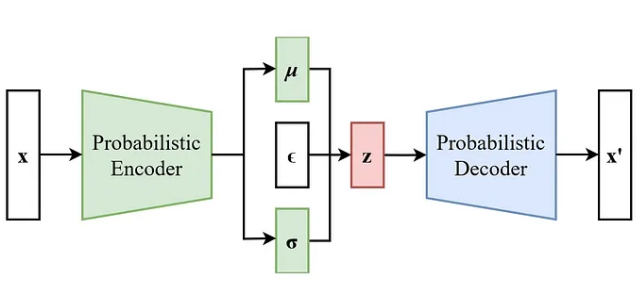
\includegraphics[width=0.7\linewidth]{1000000100000281000001274FCCAC91.png}
    \caption{VAE architecture}
    \label{fig:vae-arch}
\end{figure}

% ----
\subsection{1.2 \; Implementation}

Two VAE variants were implemented: an MLP-based model following the original paper, and a convolutional model designed for CIFAR-10 to enable a fair comparison with DDPM.

\subsubsection*{VAE-MLP}

The MLP VAE follows Appendix C.1 of Kingma \& Welling (2013) exactly, trained on MNIST ($28 \times 28$ grayscale, input dimension 784). The full architecture is shown in Figure~\ref{fig:mlp-vae}.

\begin{itemize}
    \item \textbf{Encoder:} Input $\to$ FC(400) $\to$ ReLU $\to$ FC(200) $\to$ ReLU $\to$ separate linear heads for $\mu$ and $\log\sigma^2$
    \item \textbf{Decoder:} $z \to$ FC(200) $\to$ ReLU $\to$ FC(400) $\to$ ReLU $\to$ FC(input\_size) $\to$ Sigmoid
\end{itemize}

\paperref{Paper ref --- Appendix C.1 (MNIST architecture)}

\begin{figure}[H]
\centering
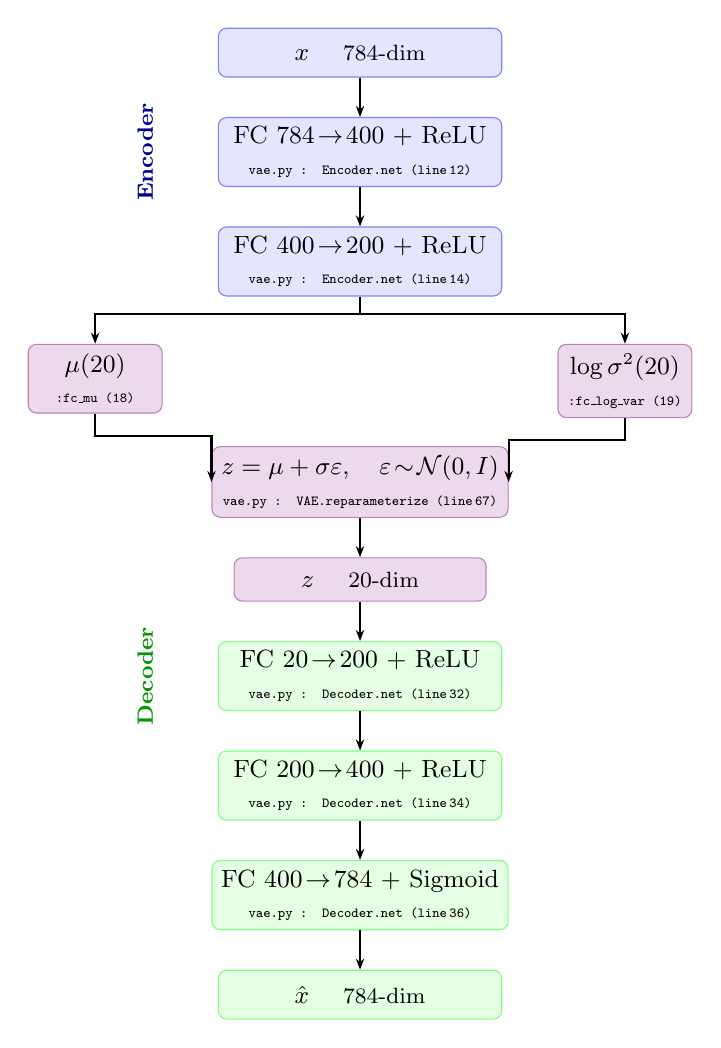
\begin{tikzpicture}[
  enc/.style  = {draw, rounded corners=3pt, fill=blue!10,   draw=blue!50,
                 minimum width=3.6cm, minimum height=0.62cm, font=\small, align=center},
  dec/.style  = {draw, rounded corners=3pt, fill=green!10,  draw=green!50,
                 minimum width=3.6cm, minimum height=0.62cm, font=\small, align=center},
  lat/.style  = {draw, rounded corners=3pt, fill=violet!15, draw=violet!50,
                 minimum width=3.2cm, minimum height=0.55cm, font=\small, align=center},
  hlat/.style = {draw, rounded corners=3pt, fill=violet!15, draw=violet!50,
                 minimum width=1.7cm, minimum height=0.55cm, font=\small, align=center},
  arr/.style  = {-{Stealth[length=4pt]}, thick},
  node distance = 0.5cm,
]

% ── Input ────────────────────────────────────────────────────────────────────
\node[enc]              (x)   {$x$ \quad \footnotesize 784-dim};

% ── Encoder layers ───────────────────────────────────────────────────────────
\node[enc, below=of x]  (e1)  {FC $784\!\to\!400$ + ReLU\\\tiny\texttt{vae.py : Encoder.net (line\,12)}};
\node[enc, below=of e1] (e2)  {FC $400\!\to\!200$ + ReLU\\\tiny\texttt{vae.py : Encoder.net (line\,14)}};

\draw[arr] (x)  -- (e1);
\draw[arr] (e1) -- (e2);

\node[font=\footnotesize\bfseries, text=blue!60!black, left=0.7cm of e1]
      {\rotatebox{90}{Encoder}};

% ── Heads: μ and log_var ─────────────────────────────────────────────────────
\node[hlat, below left =0.6cm and 0.7cm of e2] (mu)
      {$\mu(20)$\\\tiny\texttt{:fc\_mu (18)}};
\node[hlat, below right=0.6cm and 0.7cm of e2] (lv)
      {$\log\sigma^2(20)$\\\tiny\texttt{:fc\_log\_var (19)}};

\draw[arr] (e2.south) -- ++(0,-0.22) -| (mu.north);
\draw[arr] (e2.south) -- ++(0,-0.22) -| (lv.north);

% ── Reparameterize ────────────────────────────────────────────────────────────
\node[lat, below=1.9cm of e2] (rep)
      {$z = \mu + \sigma\varepsilon,\quad\varepsilon\!\sim\!\mathcal{N}(0,I)$\\\tiny\texttt{vae.py : VAE.reparameterize (line\,67)}};

\draw[arr] (mu.south) -- ++(0,-0.28) -| (rep.west);
\draw[arr] (lv.south) -- ++(0,-0.28) -| (rep.east);

% ── Latent z ──────────────────────────────────────────────────────────────────
\node[lat, below=0.5cm of rep] (z) {$z$ \quad \footnotesize 20-dim};
\draw[arr] (rep) -- (z);

% ── Decoder layers ────────────────────────────────────────────────────────────
\node[dec, below=0.5cm of z]  (d1)   {FC $20\!\to\!200$ + ReLU\\\tiny\texttt{vae.py : Decoder.net (line\,32)}};
\node[dec, below=of d1]       (d2)   {FC $200\!\to\!400$ + ReLU\\\tiny\texttt{vae.py : Decoder.net (line\,34)}};
\node[dec, below=of d2]       (d3)   {FC $400\!\to\!784$ + Sigmoid\\\tiny\texttt{vae.py : Decoder.net (line\,36)}};
\node[dec, below=of d3]       (xhat) {$\hat{x}$ \quad \footnotesize 784-dim};

\draw[arr] (z)    -- (d1);
\draw[arr] (d1)   -- (d2);
\draw[arr] (d2)   -- (d3);
\draw[arr] (d3)   -- (xhat);

\node[font=\footnotesize\bfseries, text=green!60!black, left=0.7cm of d1]
      {\rotatebox{90}{Decoder}};

\end{tikzpicture}
\caption{MLP-VAE architecture (\texttt{models/vae.py}). Encoder maps $x$ to Gaussian parameters $(\mu,\log\sigma^2)$ via \texttt{Encoder} (line~6); the reparameterization trick in \texttt{VAE.reparameterize} (line~67) samples $z = \mu+\sigma\varepsilon$ while keeping gradients flowing; the decoder in \texttt{Decoder} (line~26) reconstructs $\hat{x}$.}
\label{fig:mlp-vae}
\end{figure}

\subsubsection*{VAE-CONV}

For a fair comparison with DDPM --- which operates on CIFAR-10 ($32 \times 32$ RGB) --- a convolutional VAE was implemented on the same dataset and data normalisation ($[-1, 1]$). Using an MLP on $32 \times 32$ RGB (3,072 dims) would be prohibitively large. The architecture uses strided convolutions for downsampling (encoder) and transposed convolutions for upsampling (decoder), as shown in Figure~\ref{fig:conv-vae}.

\begin{figure}[H]
\centering
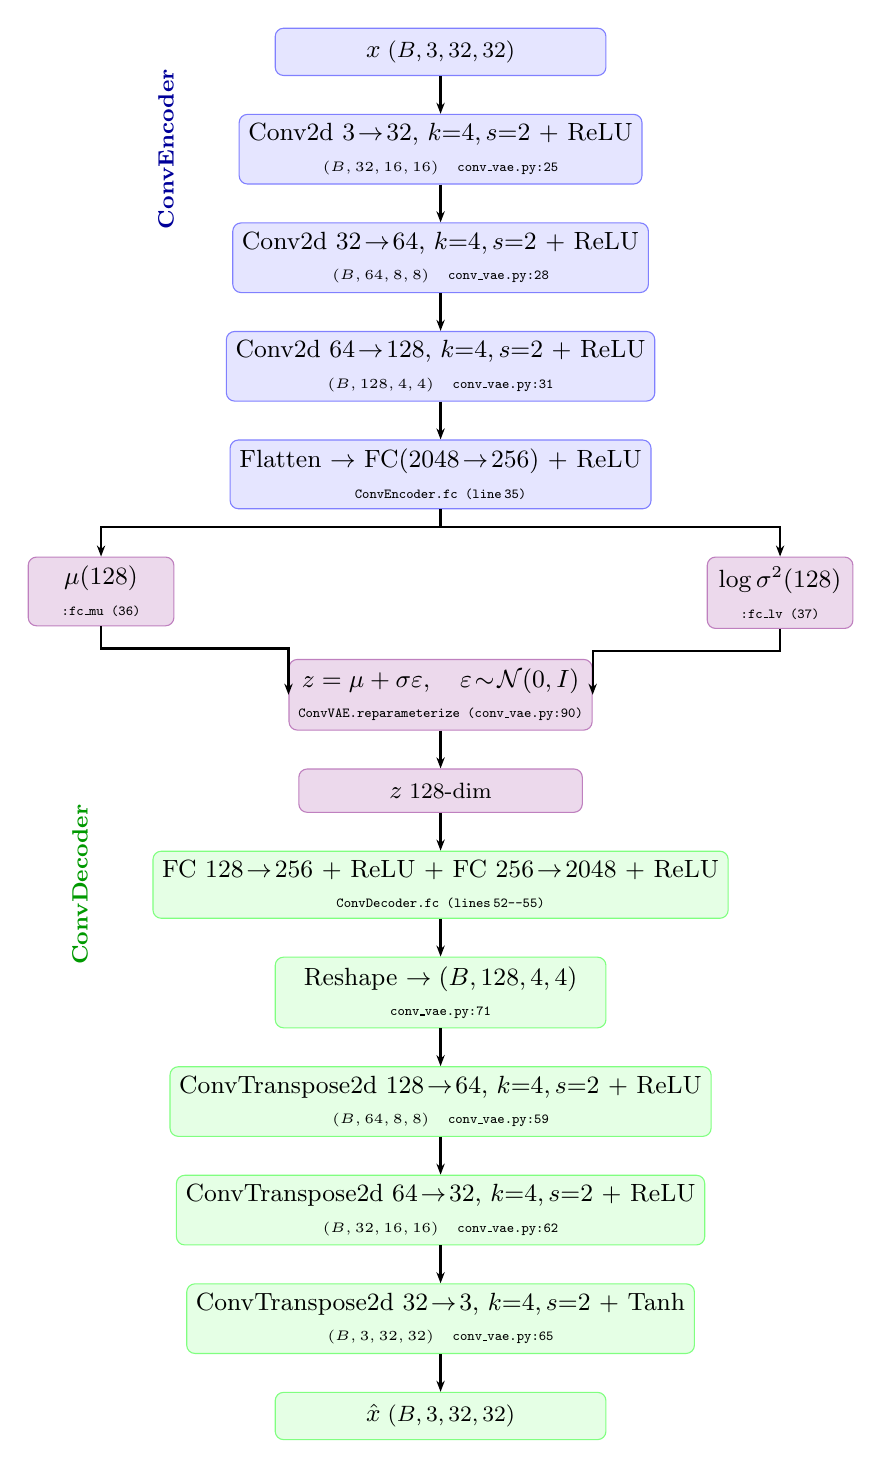
\begin{tikzpicture}[
  enc/.style  = {draw, rounded corners=3pt, fill=blue!10,   draw=blue!50,
                 minimum width=4.2cm, minimum height=0.60cm, font=\small, align=center},
  dec/.style  = {draw, rounded corners=3pt, fill=green!10,  draw=green!50,
                 minimum width=4.2cm, minimum height=0.60cm, font=\small, align=center},
  lat/.style  = {draw, rounded corners=3pt, fill=violet!15, draw=violet!50,
                 minimum width=3.6cm, minimum height=0.55cm, font=\small, align=center},
  hlat/.style = {draw, rounded corners=3pt, fill=violet!15, draw=violet!50,
                 minimum width=1.85cm, minimum height=0.55cm, font=\small, align=center},
  arr/.style  = {-{Stealth[length=4pt]}, thick},
  node distance = 0.48cm,
]

% ── Input ────────────────────────────────────────────────────────────────────
\node[enc] (x) {$x$\;\footnotesize$(B,3,32,32)$};

% ── Encoder conv layers ───────────────────────────────────────────────────────
\node[enc, below=of x]  (ec1)
    {Conv2d $3\!\to\!32$, $k{=}4,s{=}2$ + ReLU\\\tiny$(B,32,16,16)$\quad\texttt{conv\_vae.py:25}};
\node[enc, below=of ec1] (ec2)
    {Conv2d $32\!\to\!64$, $k{=}4,s{=}2$ + ReLU\\\tiny$(B,64,8,8)$\quad\texttt{conv\_vae.py:28}};
\node[enc, below=of ec2] (ec3)
    {Conv2d $64\!\to\!128$, $k{=}4,s{=}2$ + ReLU\\\tiny$(B,128,4,4)$\quad\texttt{conv\_vae.py:31}};
\node[enc, below=of ec3] (eflat)
    {Flatten $\to$ FC$(2048\!\to\!256)$ + ReLU\\\tiny\texttt{ConvEncoder.fc (line\,35)}};

\draw[arr] (x)    -- (ec1);
\draw[arr] (ec1)  -- (ec2);
\draw[arr] (ec2)  -- (ec3);
\draw[arr] (ec3)  -- (eflat);

\node[font=\footnotesize\bfseries, text=blue!60!black, left=0.7cm of ec1]
      {\rotatebox{90}{ConvEncoder}};

% ── Heads: μ and log_var ─────────────────────────────────────────────────────
\node[hlat, below left =0.6cm and 0.7cm of eflat] (mu)
      {$\mu(128)$\\\tiny\texttt{:fc\_mu (36)}};
\node[hlat, below right=0.6cm and 0.7cm of eflat] (lv)
      {$\log\sigma^2(128)$\\\tiny\texttt{:fc\_lv (37)}};

\draw[arr] (eflat.south) -- ++(0,-0.22) -| (mu.north);
\draw[arr] (eflat.south) -- ++(0,-0.22) -| (lv.north);

% ── Reparameterize ────────────────────────────────────────────────────────────
\node[lat, below=1.9cm of eflat] (rep)
      {$z = \mu + \sigma\varepsilon,\quad\varepsilon\!\sim\!\mathcal{N}(0,I)$\\\tiny\texttt{ConvVAE.reparameterize (conv\_vae.py:90)}};

\draw[arr] (mu.south) -- ++(0,-0.28) -| (rep.west);
\draw[arr] (lv.south) -- ++(0,-0.28) -| (rep.east);

% ── Latent z ──────────────────────────────────────────────────────────────────
\node[lat, below=0.48cm of rep] (z) {$z$\;\footnotesize 128-dim};
\draw[arr] (rep) -- (z);

% ── Decoder FC ────────────────────────────────────────────────────────────────
\node[dec, below=0.48cm of z] (dfc)
    {FC $128\!\to\!256$ + ReLU + FC $256\!\to\!2048$ + ReLU\\\tiny\texttt{ConvDecoder.fc (lines\,52--55)}};
\node[dec, below=of dfc] (drs)
    {Reshape $\to(B,128,4,4)$\\\tiny\texttt{conv\_vae.py:71}};

\draw[arr] (z)   -- (dfc);
\draw[arr] (dfc) -- (drs);

% ── Decoder deconv layers ─────────────────────────────────────────────────────
\node[dec, below=of drs]  (dc1)
    {ConvTranspose2d $128\!\to\!64$, $k{=}4,s{=}2$ + ReLU\\\tiny$(B,64,8,8)$\quad\texttt{conv\_vae.py:59}};
\node[dec, below=of dc1]  (dc2)
    {ConvTranspose2d $64\!\to\!32$, $k{=}4,s{=}2$ + ReLU\\\tiny$(B,32,16,16)$\quad\texttt{conv\_vae.py:62}};
\node[dec, below=of dc2]  (dc3)
    {ConvTranspose2d $32\!\to\!3$, $k{=}4,s{=}2$ + Tanh\\\tiny$(B,3,32,32)$\quad\texttt{conv\_vae.py:65}};
\node[dec, below=of dc3]  (xhat) {$\hat{x}$\;\footnotesize$(B,3,32,32)$};

\draw[arr] (drs) -- (dc1);
\draw[arr] (dc1) -- (dc2);
\draw[arr] (dc2) -- (dc3);
\draw[arr] (dc3) -- (xhat);

\node[font=\footnotesize\bfseries, text=green!60!black, left=0.7cm of dfc]
      {\rotatebox{90}{ConvDecoder}};

\end{tikzpicture}
\caption{ConvVAE architecture (\texttt{models/conv\_vae.py}). The encoder (\texttt{ConvEncoder}, line~19) uses three stride-2 Conv2d layers to compress $(B,3,32,32)$ to $(B,128,4,4)$, then a FC layer produces $\mu$ and $\log\sigma^2$. Reparameterization (\texttt{ConvVAE.reparameterize}, line~90) samples $z\in\mathbb{R}^{128}$. The decoder (\texttt{ConvDecoder}, line~46) mirrors the encoder with transposed convolutions, outputting $\hat{x}\in[-1,1]$ via Tanh.}
\label{fig:conv-vae}
\end{figure}

\subsubsection*{KL Divergence --- Closed Form}

For Gaussian encoder $q(z|x) = \mathcal{N}(\mu, \sigma^2 I)$ and prior $p(z) = \mathcal{N}(0, I)$, the KL divergence has a closed form --- no sampling needed:
\[
D_{\mathrm{KL}} = -\frac{1}{2}\sum_{j=1}^{J}\left(1 + \log\sigma_j^2 - \mu_j^2 - \sigma_j^2\right)
\]

\paperref{Paper ref --- Appendix B, Equation B.3.}

\subsubsection*{Reconstruction Loss --- Two Variants}

\begin{itemize}
    \item \textbf{MNIST:} pixel values are binary $\to$ $p(x|z)$ modeled as Bernoulli $\to$ Binary Cross-Entropy loss
    \item \textbf{Frey Face:} pixel values are continuous $\to$ $p(x|z)$ modeled as Gaussian $\to$ MSE loss
\end{itemize}

\paperref{Paper ref --- Appendix C.1 (Bernoulli MLP for MNIST), Appendix C.2 (Gaussian MLP for Frey Face).}

% ----
\subsection{1.3 \; Training Configuration}

\subsubsection*{Dataset 1 --- MNIST}

MNIST contains 60,000 grayscale handwritten digit images ($28 \times 28$ pixels). Since pixel values represent ink intensity in $[0,1]$, they are treated as Bernoulli probabilities $\to$ BCE loss.

\begin{table}[H]
\centering
\caption{VAE-MLP Training Settings (MNIST)}
\begin{tabular}{lll}
\toprule
\textbf{Setting} & \textbf{Value} & \textbf{Paper source} \\
\midrule
Input dimension       & 784 ($28{\times}28$)   & Appendix C.1 \\
Latent dimension      & 20                      & Appendix C.1: ``$L = 20$'' \\
Hidden dimension      & 400                     & Appendix C.1 (200 in paper; 400 used here) \\
Reconstruction loss   & BCE (Bernoulli)         & Appendix C.1 \\
Optimizer             & Adam, lr=$10^{-3}$      & Section 5 / Appendix C \\
Batch size            & 128                     & Appendix C \\
Epochs                & 50                      & --- \\
\bottomrule
\end{tabular}
\end{table}

\paperref{Paper ref --- Appendix C.1: ``We used \ldots\ a Bernoulli MLP as decoder.''}

% ----
\subsection{1.4 \; Results}

The VAE-MLP is evaluated separately to show the concept.

\subsubsection*{MNIST --- Reconstructions}

The model learns to reconstruct digits cleanly within a few epochs. By epoch 10 the outputs are recognizable; by epoch 50 they are accurate, as shown in Figure~\ref{fig:vae-recon}.

\begin{figure}[H]
    \centering
    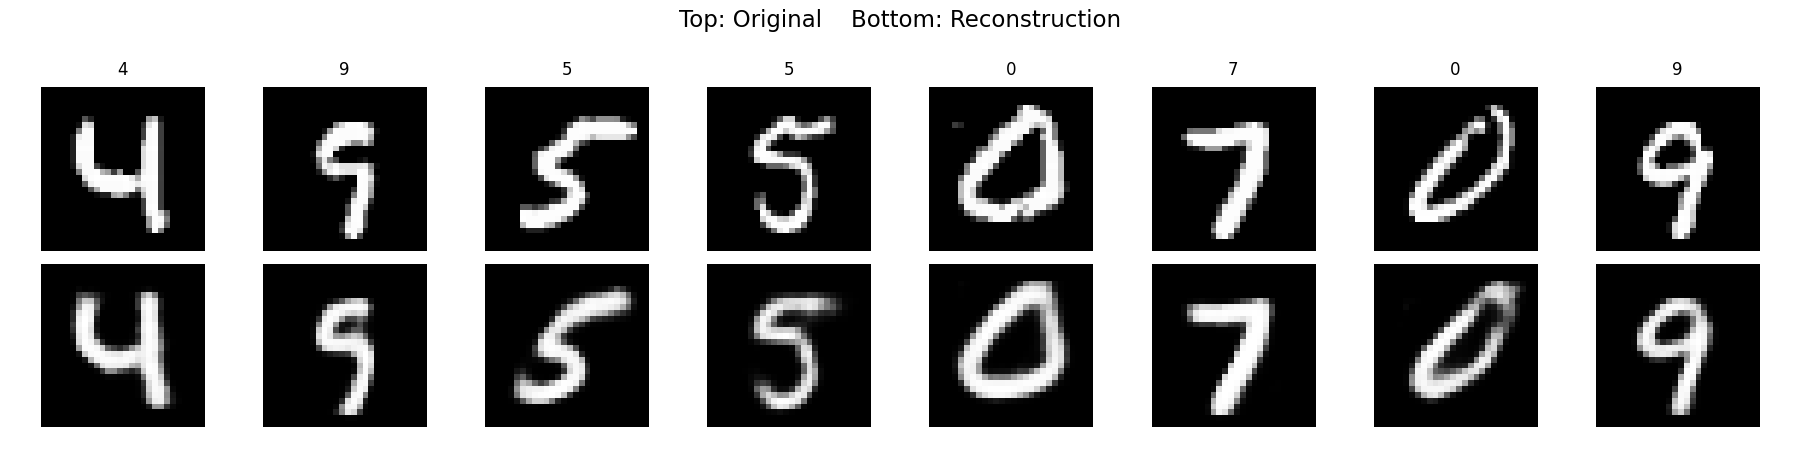
\includegraphics[width=0.7\linewidth]{1000000100000708000001C296CA6C8F.png}
    \caption{VAE reconstructions on MNIST (top: original, bottom: reconstructed)}
    \label{fig:vae-recon}
\end{figure}

\subsubsection*{MNIST --- Generated Samples}

Sampling by drawing $z \sim \mathcal{N}(0, I)$ and decoding produces plausible digits, as shown in Figure~\ref{fig:vae-samples}. Samples are somewhat blurry compared to real images --- a known limitation of VAEs. The reconstruction loss favors pixel-level accuracy over sharpness.

\begin{figure}[H]
    \centering
    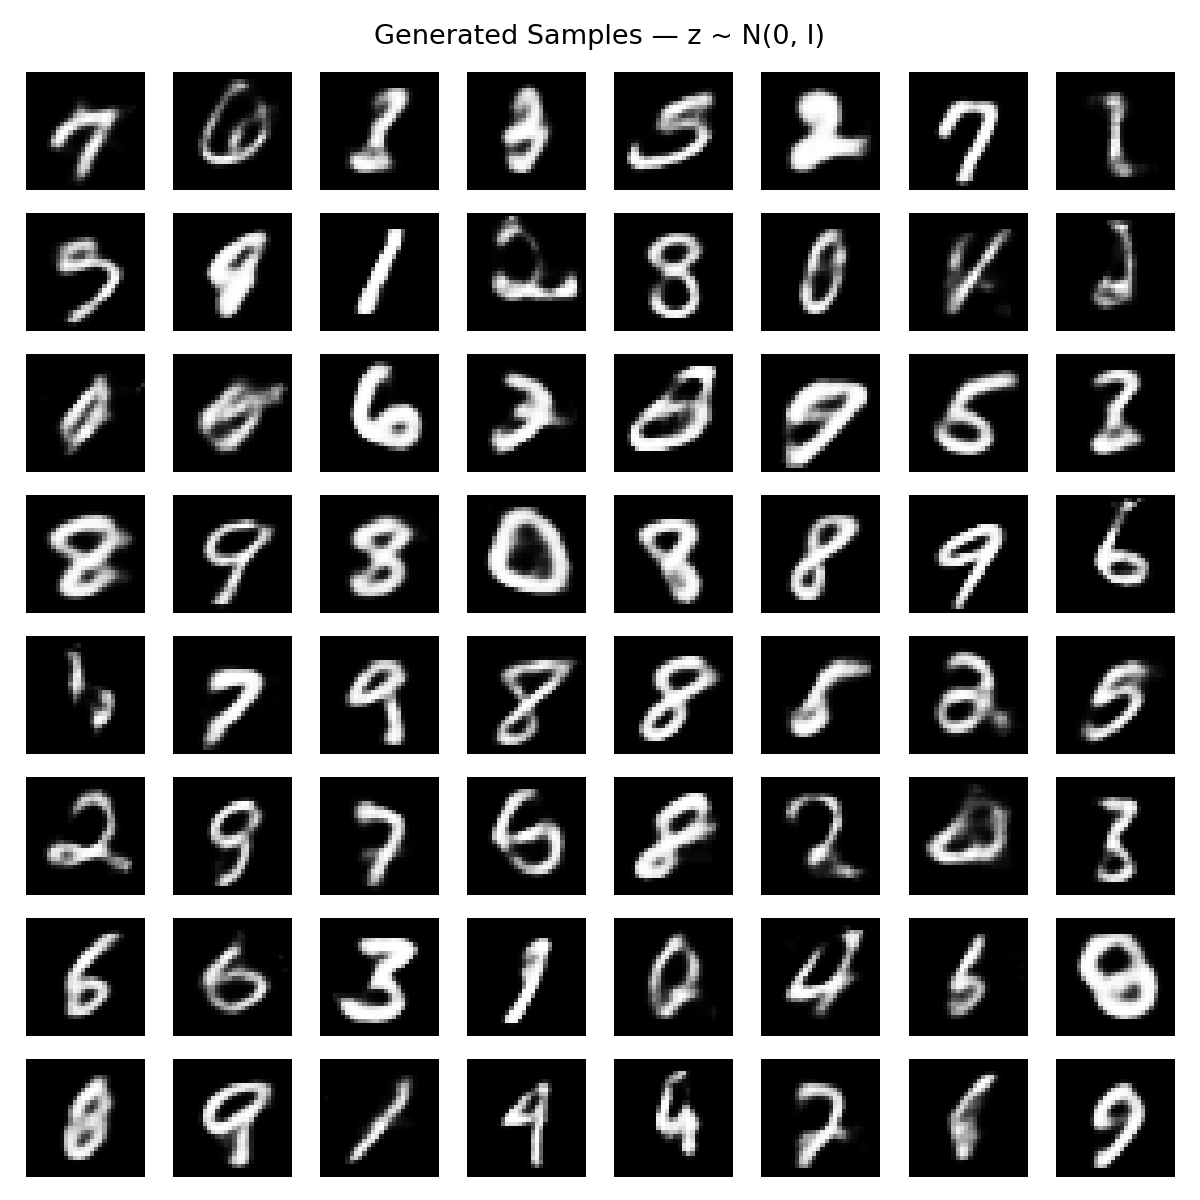
\includegraphics[width=0.7\linewidth]{10000001000004B0000004B01AF43090.png}
    \caption{Random samples generated by the VAE from MNIST latent space}
    \label{fig:vae-samples}
\end{figure}

\subsubsection*{MNIST --- Latent Space Interpolation}

Linearly interpolating between two points in latent space produces smooth transitions between digits, as shown in Figure~\ref{fig:vae-interp}. This demonstrates the KL regularization working as intended --- the latent space is continuous and meaningful.

\begin{figure}[H]
    \centering
    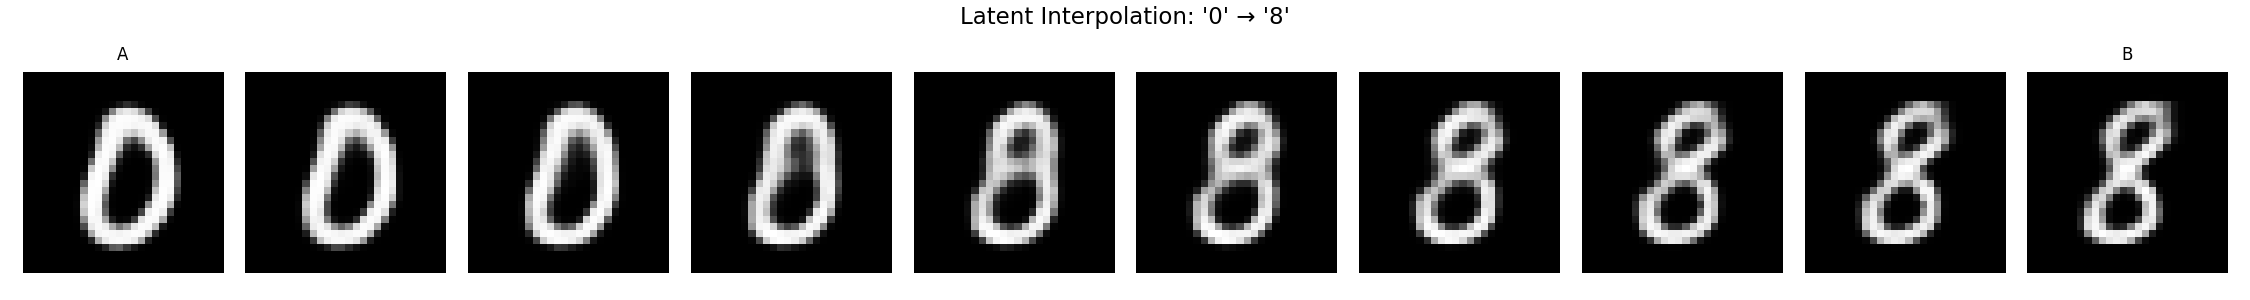
\includegraphics[width=0.8\linewidth]{10000001000008CA0000012C9F93D100.png}
    \caption{Smooth interpolation between digit pairs in the 20-dim latent space}
    \label{fig:vae-interp}
\end{figure}

\paperref{Paper ref --- Section 3: ``The KL term encourages the encoder to be close to the prior, making the latent space \ldots''}

\newpage
% ============================================================
\section{Part 2 --- Denoising Diffusion Probabilistic Model (DDPM)}
% ============================================================

\subsection{2.1 \; Theoretical Background}

A DDPM takes a completely different approach to generative modeling. Instead of learning a compressed representation, it learns to reverse a gradual noising process. The model defines two paired Markov chains: a fixed forward process $q$ that gradually adds noise to data, and a learned reverse process $p_\theta$ that denoises, as illustrated in Figure~\ref{fig:ddpm-overview}.

\begin{figure}[H]
    \centering
    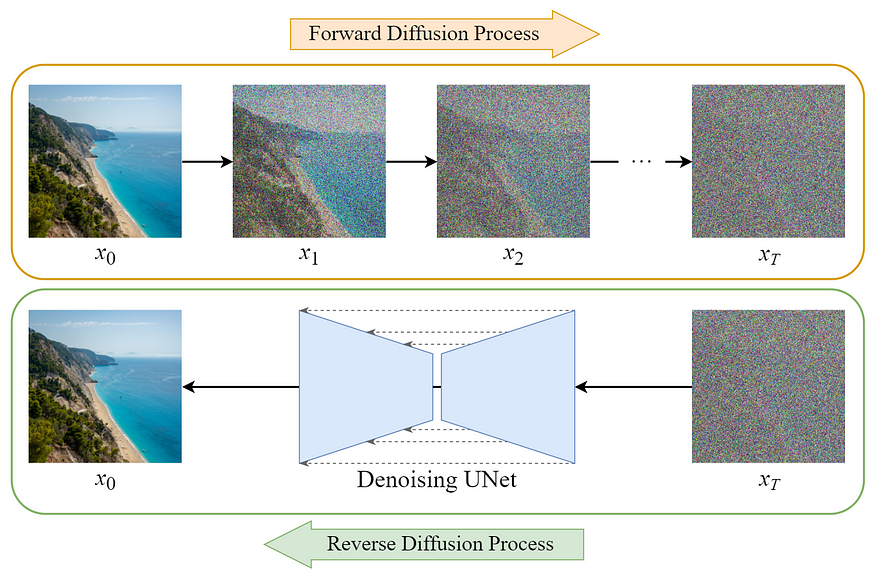
\includegraphics[width=0.85\linewidth]{100000010000036B000002434198030D.png}
    \caption{Overview of the diffusion model: forward process $q$ (left$\to$right) and reverse process $p_\theta$ (right$\to$left)}
    \label{fig:ddpm-overview}
\end{figure}

\subsection{2.2 \; Forward Process}

The forward process $q$ gradually corrupts a real image by adding small amounts of Gaussian noise at each of $T=1000$ timesteps until the image becomes pure noise. The variance schedule is fixed --- it is not learned. Using the reparameterization with $\bar{\alpha}_t = \prod \alpha_s$ (cumulative product), any timestep $t$ can be reached in one shot without iterating step by step, as shown in Figure~\ref{fig:forward-process}:
\[
q(x_t | x_0) = \mathcal{N}(x_t;\, \sqrt{\bar{\alpha}_t}\,x_0,\; (1 - \bar{\alpha}_t)\,I)
\]

\paperref{Paper ref --- Section 2, Equations 2 and 4. This closed form is what makes training efficient.}

\begin{figure}[H]
    \centering
    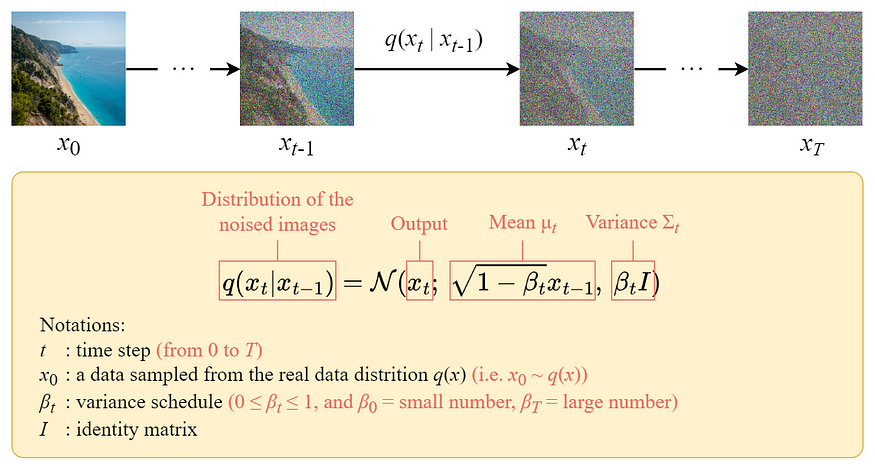
\includegraphics[width=0.85\linewidth]{100000010000036B000001D677227387.png}
    \caption{Forward diffusion process: clean image $x_0$ is gradually corrupted over $T=1000$ steps}
    \label{fig:forward-process}
\end{figure}

Representative training examples used during the CIFAR-10 run are shown in Figure~\ref{fig:training-data}.

\begin{figure}[H]
    \centering
    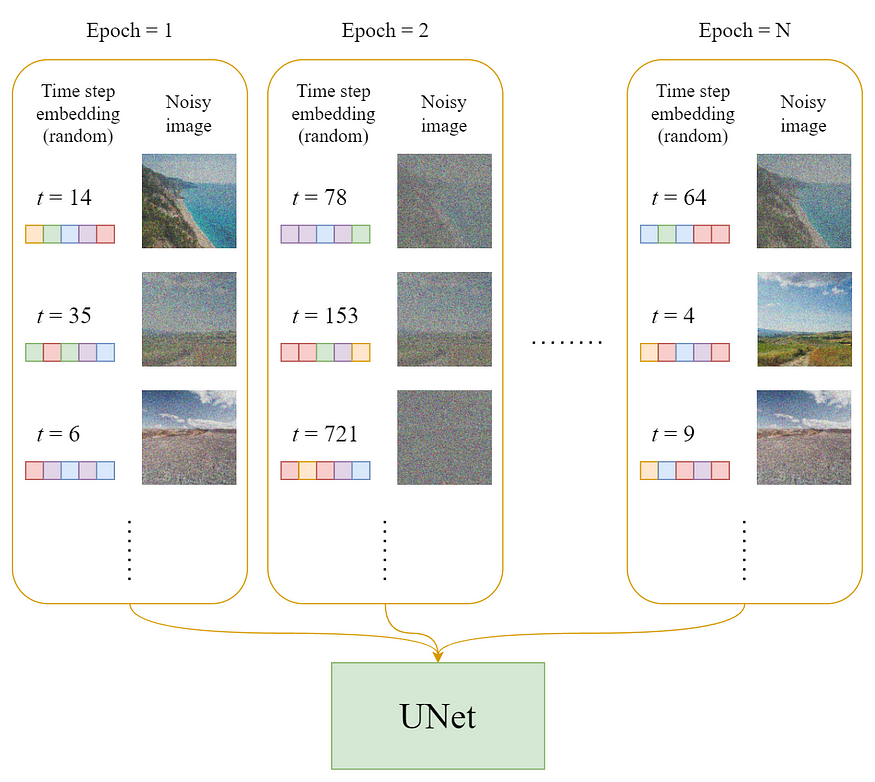
\includegraphics[width=0.85\linewidth]{100000010000036B0000030EADF9BFF1.png}
    \caption{Examples of the training data used for the diffusion model}
    \label{fig:training-data}
\end{figure}

The noise schedule controls how quickly the image is corrupted. A linear schedule is used, increasing $\beta_t$ from a very small value at $t=1$ to $0.02$ at $t=T$.

\paperref{Paper ref --- Section 4: ``We set $T = 1000$ \ldots\ forward process variances to constants increasing linearly from $\beta_1 = 10^{-4}$ to $\beta_T = 0.02$.''}

\subsection{2.3 \; Model Architecture (U-Net)}

The reverse process is parameterized by a U-Net that takes a noisy image $x_t$ and timestep $t$ as input, and predicts the noise $\varepsilon$ that was added. The U-Net has four resolution levels ($32{\times}32 \to 16{\times}16 \to 8{\times}8 \to 4{\times}4$) with skip connections, as shown in Figure~\ref{fig:unet-arch}.

\begin{figure}[H]
\centering
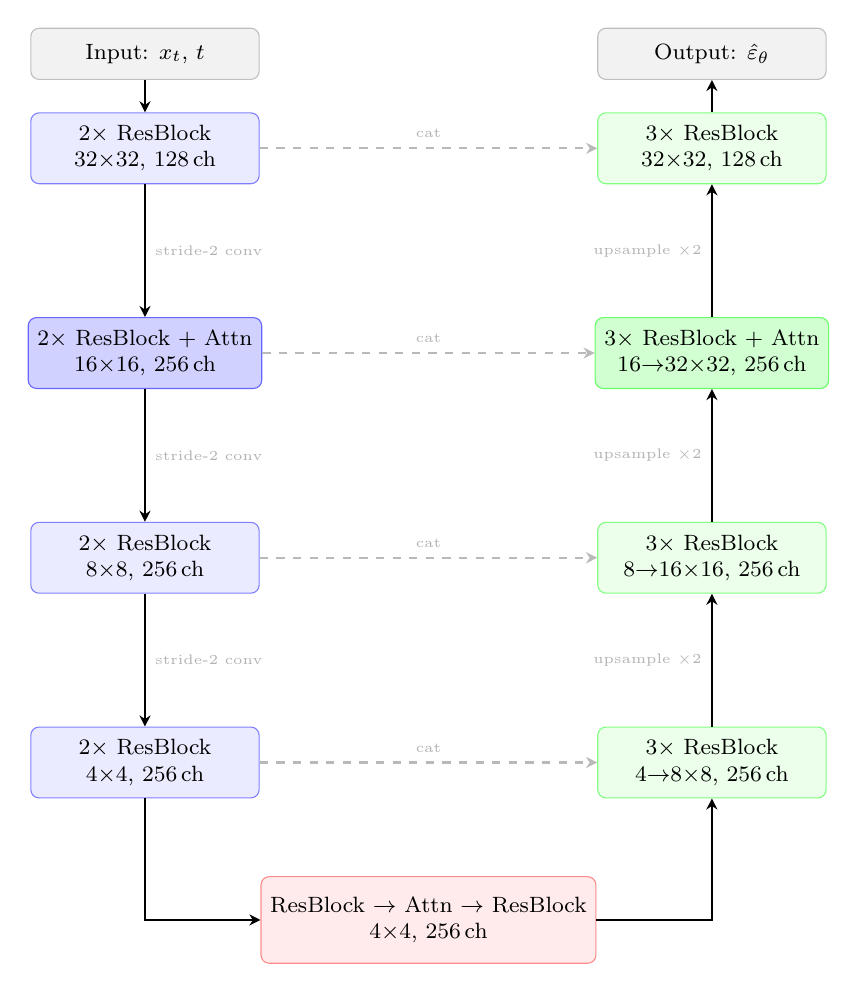
\begin{tikzpicture}[
    every node/.style = {align=center},
    encbox/.style  = {draw, rounded corners=3pt, fill=blue!8,   draw=blue!50,
                      minimum width=2.9cm, minimum height=0.9cm,  font=\footnotesize},
    decbox/.style  = {draw, rounded corners=3pt, fill=green!8,  draw=green!50,
                      minimum width=2.9cm, minimum height=0.9cm,  font=\footnotesize},
    encattn/.style = {draw, rounded corners=3pt, fill=blue!18,  draw=blue!60,
                      minimum width=2.9cm, minimum height=0.9cm,  font=\footnotesize},
    decattn/.style = {draw, rounded corners=3pt, fill=green!18, draw=green!60,
                      minimum width=2.9cm, minimum height=0.9cm,  font=\footnotesize},
    botbox/.style  = {draw, rounded corners=3pt, fill=red!8,    draw=red!45,
                      minimum width=2.9cm, minimum height=1.1cm,  font=\footnotesize},
    iobox/.style   = {draw, rounded corners=3pt, fill=gray!10,  draw=gray!50,
                      minimum width=2.9cm, minimum height=0.65cm, font=\footnotesize},
    arr/.style     = {-{Stealth[length=4pt,width=4pt]}, thick},
    skip/.style    = {-{Stealth[length=4pt,width=4pt]}, thick, dashed, draw=gray!55},
    slabel/.style  = {font=\tiny, text=gray!60},
]

%% IO
\node[iobox] (input)  at (0cm,     1.2cm)  {Input: $x_t$,\ $t$};
\node[iobox] (output) at (7.2cm,   1.2cm)  {Output: $\hat{\varepsilon}_\theta$};

%% Encoder
\node[encbox]  (e0) at (0cm,   0cm)    {2$\times$ ResBlock\\$32{\times}32$,\ 128\,ch};
\node[encattn] (e1) at (0cm,  -2.6cm)  {2$\times$ ResBlock $+$ Attn\\$16{\times}16$,\ 256\,ch};
\node[encbox]  (e2) at (0cm,  -5.2cm)  {2$\times$ ResBlock\\$8{\times}8$,\ 256\,ch};
\node[encbox]  (e3) at (0cm,  -7.8cm)  {2$\times$ ResBlock\\$4{\times}4$,\ 256\,ch};

%% Bottleneck
\node[botbox] (bot) at (3.6cm, -9.8cm)
    {ResBlock $\to$ Attn $\to$ ResBlock\\$4{\times}4$,\ 256\,ch};

%% Decoder
\node[decbox]  (d3) at (7.2cm, -7.8cm) {3$\times$ ResBlock\\$4{\to}8{\times}8$,\ 256\,ch};
\node[decbox]  (d2) at (7.2cm, -5.2cm) {3$\times$ ResBlock\\$8{\to}16{\times}16$,\ 256\,ch};
\node[decattn] (d1) at (7.2cm, -2.6cm) {3$\times$ ResBlock $+$ Attn\\$16{\to}32{\times}32$,\ 256\,ch};
\node[decbox]  (d0) at (7.2cm,  0cm)   {3$\times$ ResBlock\\$32{\times}32$,\ 128\,ch};

%% Encoder flow
\draw[arr] (input.south) -- (e0.north);
\draw[arr] (e0) -- node[right, slabel] {stride-2 conv} (e1);
\draw[arr] (e1) -- node[right, slabel] {stride-2 conv} (e2);
\draw[arr] (e2) -- node[right, slabel] {stride-2 conv} (e3);
\draw[arr] (e3.south) |- (bot.west);

%% Bottleneck to decoder
\draw[arr] (bot.east) -| (d3.south);
\draw[arr] (d3) -- node[left, slabel] {upsample $\times 2$} (d2);
\draw[arr] (d2) -- node[left, slabel] {upsample $\times 2$} (d1);
\draw[arr] (d1) -- node[left, slabel] {upsample $\times 2$} (d0);
\draw[arr] (d0.north) -- (output.south);

%% Skip connections
\draw[skip] (e0.east) -- node[above, slabel] {cat} (d0.west);
\draw[skip] (e1.east) -- node[above, slabel] {cat} (d1.west);
\draw[skip] (e2.east) -- node[above, slabel] {cat} (d2.west);
\draw[skip] (e3.east) -- node[above, slabel] {cat} (d3.west);

\end{tikzpicture}
\caption{U-Net backbone $\varepsilon_\theta(x_t,t)$ (\texttt{models/ddpm.py : UNet}). \textcolor{blue!60!black}{Blue}: encoder, downsamples via stride-2 conv. \textcolor{red!50!black}{Red}: bottleneck. \textcolor{green!50!black}{Green}: decoder, upsamples via nearest-neighbour $+$ conv. Dashed arrows: skip connections (channel-wise concatenation). Darker shading marks levels with self-attention ($16{\times}16$ resolution only). Implementation: \texttt{UNet.\_\_init\_\_} (line~171), \texttt{UNet.forward} (line~264).}
\label{fig:unet-arch}
\end{figure}

\paperref{Paper ref --- Appendix B: ``Our neural network architecture follows the backbone of PixelCNN++ \ldots\ a U-Net based on a Wide ResNet. Our $32{\times}32$ models use four feature map resolutions (\ldots) and all models have two convolutional residual blocks per resolution level.''}

\subsubsection*{Component 1 --- Time Embedding}

The scalar timestep $t$ must be communicated to the network so every block knows which noise level it is working with. A sinusoidal positional embedding (borrowed from Transformers) encodes $t$ into a rich 128-dim vector, which is then projected to 256 dims and injected into every ResBlock, as shown in Figure~\ref{fig:time-emb}.

\begin{figure}[H]
\centering
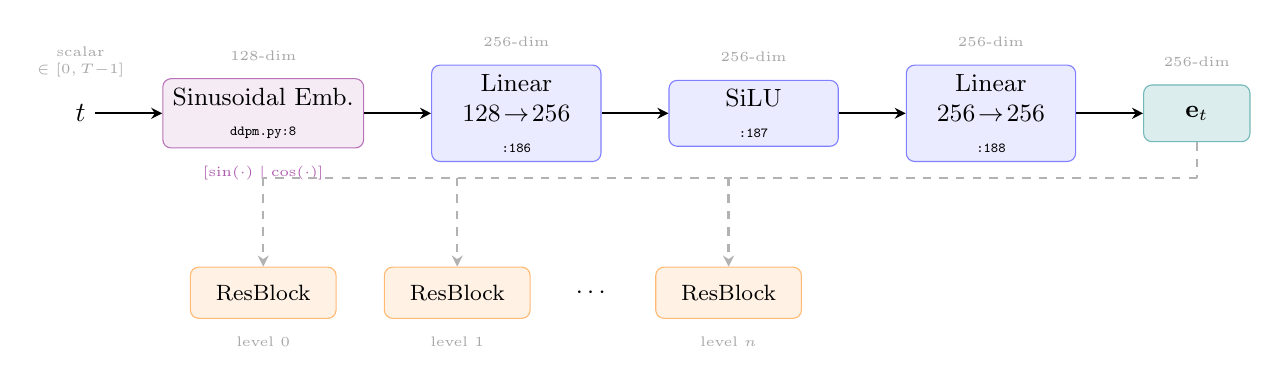
\begin{tikzpicture}[
    node distance = 0.45cm and 0.85cm,
    every node/.style = {align=center},
    block/.style    = {draw, rounded corners=3pt, fill=blue!8,   draw=blue!50,
                       minimum width=2.15cm, minimum height=0.72cm, font=\small},
    sinblock/.style = {draw, rounded corners=3pt, fill=violet!8, draw=violet!55,
                       minimum width=2.55cm, minimum height=0.72cm, font=\small},
    outblock/.style = {draw, rounded corners=3pt, fill=teal!14,  draw=teal!55,
                       minimum width=1.35cm, minimum height=0.72cm,
                       font=\small\bfseries},
    resblock/.style = {draw, rounded corners=3pt, fill=orange!10, draw=orange!55,
                       minimum width=1.85cm, minimum height=0.65cm, font=\footnotesize},
    arr/.style      = {-{Stealth[length=4pt,width=4pt]}, thick},
    iarr/.style     = {-{Stealth[length=4pt,width=4pt]}, thick, dashed, draw=gray!60},
    dlabel/.style   = {font=\tiny, text=gray!70},
]

%% Input node
\node (t) {$t$};
\node[dlabel, above=3pt of t] {scalar\\$\in[0,T{-}1]$};

%% Pipeline
\node[sinblock, right=0.85cm of t]   (se)  {Sinusoidal Emb.\\\tiny\texttt{ddpm.py:8}};
\node[block,    right=0.85cm of se]  (l1)  {Linear\\$128\!\to\!256$\\\tiny\texttt{:186}};
\node[block,    right=0.85cm of l1]  (act) {SiLU\\\tiny\texttt{:187}};
\node[block,    right=0.85cm of act] (l2)  {Linear\\$256\!\to\!256$\\\tiny\texttt{:188}};
\node[outblock, right=0.85cm of l2]  (out) {$\mathbf{e}_t$};

%% Dimension labels above each node
\node[dlabel, above=3pt of se]  {128-dim};
\node[dlabel, above=3pt of l1]  {256-dim};
\node[dlabel, above=3pt of act] {256-dim};
\node[dlabel, above=3pt of l2]  {256-dim};
\node[dlabel, above=3pt of out] {256-dim};

%% Detail label below sinusoidal box
\node[font=\tiny\itshape, text=violet!65, below=3pt of se]
    {$[\sin(\cdot)\mid\cos(\cdot)]$};

%% Main arrows
\draw[arr] (t)   -- (se);
\draw[arr] (se)  -- (l1);
\draw[arr] (l1)  -- (act);
\draw[arr] (act) -- (l2);
\draw[arr] (l2)  -- (out);

%% ResBlock row (below the pipeline)
\node[resblock, below=1.5cm of se]    (rb0)  {ResBlock};
\node[resblock, right=0.6cm of rb0]   (rb1)  {ResBlock};
\node[font=\small, right=0.45cm of rb1] (dots) {$\cdots$};
\node[resblock, right=0.45cm of dots] (rbn)  {ResBlock};

\node[dlabel, below=3pt of rb0] {level 0};
\node[dlabel, below=3pt of rb1] {level 1};
\node[dlabel, below=3pt of rbn] {level $n$};

%% Dashed injection: drop from e_t, horizontal bus, then down to each block
\coordinate (drop) at ($(out.south)+(0,-0.45)$);
\draw[thick, dashed, draw=gray!60] (out.south) -- (drop);
\draw[thick, dashed, draw=gray!60] (drop) -- (drop -| rb0.north);
\draw[iarr] (drop -| rb0.north) -- (rb0.north);
\draw[iarr] (drop -| rb1.north) -- (rb1.north);
\draw[iarr] (drop -| rbn.north) -- (rbn.north);

\end{tikzpicture}
\caption{Time embedding (\texttt{ddpm.py:8}, \texttt{time\_mlp:184}). Scalar $t$ is sinusoidally embedded to 128-dim, projected by two FC layers to 256-dim $\mathbf{e}_t$, and broadcast into every ResBlock.}
\label{fig:time-emb}
\end{figure}

\paperref{Paper ref --- Appendix B: ``Diffusion time $t$ is specified by adding the Transformer sinusoidal position embedding [60] into each residual block.'' Reference [60] is Vaswani et al.\ (2017).}

\subsubsection*{Component 2 --- Residual Block}

The residual block is the core building unit of the U-Net. It applies two convolutions with a skip connection, and injects the time embedding between the two convolutions so every block is aware of the current noise level, as illustrated in Figure~\ref{fig:res-block}.

\begin{figure}[H]
\centering
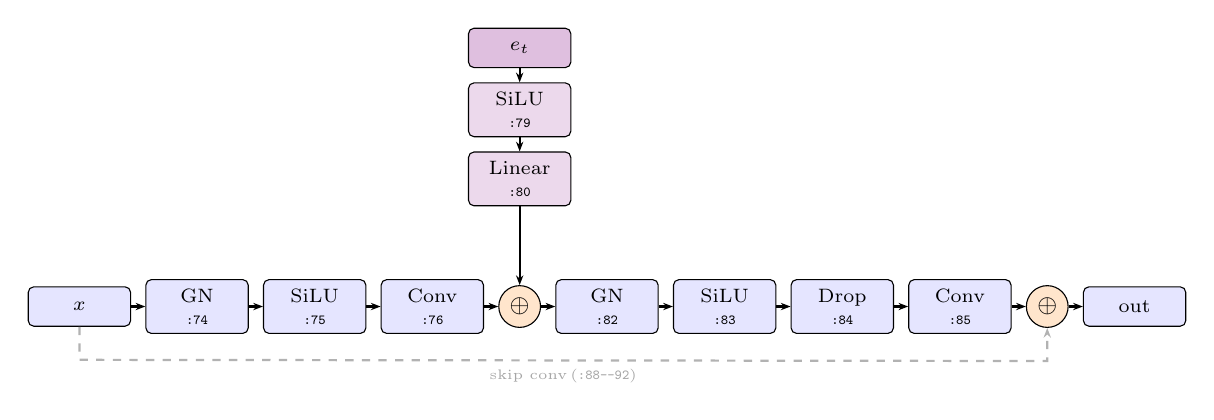
\begin{tikzpicture}[
  box/.style  = {draw, rounded corners=2pt, minimum width=1.3cm, minimum height=0.5cm,
                 align=center, fill=blue!10, font=\scriptsize},
  tbox/.style = {draw, rounded corners=2pt, minimum width=1.3cm, minimum height=0.5cm,
                 align=center, fill=violet!15, font=\scriptsize},
  addcirc/.style = {draw, circle, inner sep=2pt, fill=orange!20, font=\small},
  arr/.style  = {-{Stealth[length=3.5pt]}, thick},
]
% ── Main horizontal path ─────────────────────────────────────────────────────
\node[box]     (x)     {$x$};
\node[box,     right=0.18cm of x]     (gn1)   {GN\\\tiny\texttt{:74}};
\node[box,     right=0.18cm of gn1]   (silu1) {SiLU\\\tiny\texttt{:75}};
\node[box,     right=0.18cm of silu1] (conv1) {Conv\\\tiny\texttt{:76}};
\node[addcirc, right=0.18cm of conv1] (add1)  {$\oplus$};
\node[box,     right=0.18cm of add1]  (gn2)   {GN\\\tiny\texttt{:82}};
\node[box,     right=0.18cm of gn2]   (silu2) {SiLU\\\tiny\texttt{:83}};
\node[box,     right=0.18cm of silu2] (drop)  {Drop\\\tiny\texttt{:84}};
\node[box,     right=0.18cm of drop]  (conv2) {Conv\\\tiny\texttt{:85}};
\node[addcirc, right=0.18cm of conv2] (add2)  {$\oplus$};
\node[box,     right=0.18cm of add2]  (out)   {out};

\foreach \a/\b in {x/gn1, gn1/silu1, silu1/conv1, conv1/add1,
                   add1/gn2, gn2/silu2, silu2/drop, drop/conv2, conv2/add2, add2/out}
  \draw[arr] (\a) -- (\b);

% ── Time embedding branch (above add1) ───────────────────────────────────────
\node[tbox,              above=1.0cm of add1] (lin)   {Linear\\\tiny\texttt{:80}};
\node[tbox,              above=0.18cm of lin] (tsilu) {SiLU\\\tiny\texttt{:79}};
\node[tbox, fill=violet!25, above=0.18cm of tsilu] (et) {$e_t$};

\draw[arr] (et.south) -- (tsilu.north);
\draw[arr] (tsilu.south) -- (lin.north);
\draw[arr] (lin.south) -- (add1.north);

% ── Skip bypass (below) ───────────────────────────────────────────────────────
\coordinate (bl) at ($(x.south)+(0,-0.42)$);
\coordinate (br) at ($(add2.south)+(0,-0.42)$);
\draw[-{Stealth[length=3.5pt]}, thick, dashed, draw=gray!60]
    (x.south) -- (bl) -- (br) -- (add2.south);
\node[font=\tiny, text=gray!70] at ($(bl)!0.5!(br)+(0,-0.2)$)
    {skip conv\,(\texttt{:88--92})};
\end{tikzpicture}
\caption{Residual block data flow (\texttt{models/ddpm.py : ResidualBlock}, line~48). Two Conv\,$3{\times}3$ blocks with GroupNorm and SiLU. Time embedding $e_t$ injected via SiLU+Linear (lines~79--80) at the middle $\oplus$. Skip $1{\times}1$ conv (lines~88--92) when channels differ. Line numbers: \texttt{ResidualBlock.forward} (line~94).}
\label{fig:res-block}
\end{figure}

\begin{itemize}
    \item GroupNorm replaces weight normalization for better training stability.
    \item SiLU activation provides smooth gradient flow.
    \item Dropout rate $= 0.1$ applied to the second convolution.
    \item $1{\times}1$ skip conv when input/output channels differ; Identity otherwise.
\end{itemize}

\paperref{Paper ref --- Appendix B: ``We replaced weight normalization [49] with group normalization [66].'' Section 4: ``We set the dropout rate on CIFAR10 to 0.1.''}

\subsubsection*{Component 3 --- Self-Attention Block}

Self-attention is inserted at the $16{\times}16$ resolution only. It lets the network look at the entire feature map at once and capture long-range spatial structure --- important for generating images where distant regions must be globally consistent, as shown in Figure~\ref{fig:self-attn}.

\begin{figure}[H]
\centering
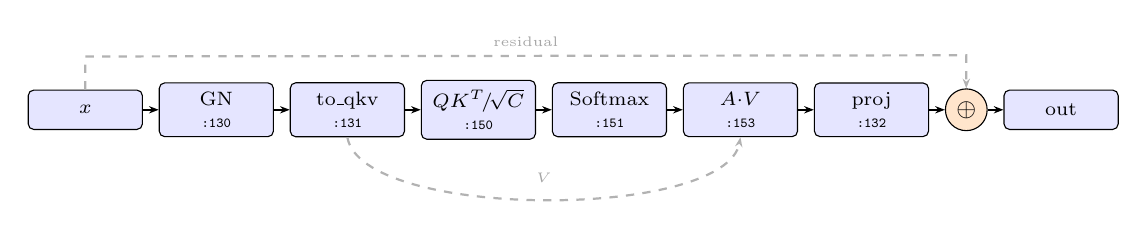
\begin{tikzpicture}[
  box/.style   = {draw, rounded corners=2pt, minimum width=1.45cm, minimum height=0.5cm,
                  align=center, fill=blue!10, font=\scriptsize},
  addcirc/.style = {draw, circle, inner sep=2pt, fill=orange!20, font=\small},
  arr/.style   = {-{Stealth[length=3.5pt]}, thick},
  darr/.style  = {-{Stealth[length=3.5pt]}, thick, dashed, draw=gray!60},
]
% ── Main horizontal path ─────────────────────────────────────────────────────
\node[box]     (x)       {$x$};
\node[box,     right=0.2cm of x]       (gn)     {GN\\\tiny\texttt{:130}};
\node[box,     right=0.2cm of gn]      (qkv)    {to\_qkv\\\tiny\texttt{:131}};
\node[box,     right=0.2cm of qkv]     (scores) {$QK^T\!/\!\sqrt{C}$\\\tiny\texttt{:150}};
\node[box,     right=0.2cm of scores]  (softmax){Softmax\\\tiny\texttt{:151}};
\node[box,     right=0.2cm of softmax] (wsum)   {$A{\cdot}V$\\\tiny\texttt{:153}};
\node[box,     right=0.2cm of wsum]    (proj)   {proj\\\tiny\texttt{:132}};
\node[addcirc, right=0.2cm of proj]    (add)    {$\oplus$};
\node[box,     right=0.2cm of add]     (out)    {out};

\foreach \a/\b in {x/gn, gn/qkv, qkv/scores, scores/softmax, softmax/wsum, wsum/proj, proj/add, add/out}
  \draw[arr] (\a) -- (\b);

% ── V bypass (arc below: qkv → wsum, skipping scores+softmax) ────────────────
\draw[darr] (qkv.south) to[out=-80, in=-100, looseness=0.55] (wsum.south);
\node[font=\tiny, text=gray!70] at ($(qkv.south)!0.5!(wsum.south)+(0,-0.52)$) {$V$};

% ── Residual skip (above, x → add) ───────────────────────────────────────────
\coordinate (sr1) at ($(x.north)+(0,0.42)$);
\coordinate (sr2) at ($(add.north)+(0,0.42)$);
\draw[darr] (x.north) -- (sr1) -- (sr2) -- (add.north);
\node[font=\tiny, text=gray!70] at ($(sr1)!0.5!(sr2)+(0,0.18)$) {residual};
\end{tikzpicture}
\caption{Self-attention block (\texttt{models/ddpm.py : AttentionBlock}, line~119). GN (line~130) $\to$ \texttt{to\_qkv} Conv\,$1{\times}1$ (line~131) splits into $Q$/$K$/$V$ $\to$ scaled dot-product $QK^T\!/\!\sqrt{C}$ (line~150) $\to$ Softmax (line~151) $\to$ $A{\cdot}V$ weighted sum (line~153) $\to$ \texttt{proj} (line~132) $\to$ residual add (line~156). $V$ bypasses the score path (dashed arc). Applied at $16{\times}16$ only; see \texttt{AttentionBlock.forward} (line~135).}
\label{fig:self-attn}
\end{figure}

\paperref{Paper ref --- Appendix B: ``We use self-attention at the $16{\times}16$ feature map resolution between the convolutional blocks.''}

\subsection{2.4 \; Training}

The model is trained on a simplified loss derived from the variational lower bound. For each training step: sample a random timestep $t$, corrupt the image to $x_t$ using Eq.\ 4, run the U-Net to predict the noise $\hat{\varepsilon}$, and minimize:
\[
\mathcal{L}_{\text{simple}} = \mathbb{E}_{t,x_0,\varepsilon}\!\left[\|\varepsilon - \varepsilon_\theta(x_t, t)\|^2\right]
\]
The full training procedure is given in Figure~\ref{fig:training-alg}, and a single training step is illustrated in Figure~\ref{fig:training-step}.

\begin{figure}[H]
\centering
\begin{minipage}{0.72\linewidth}
{\small
\noindent\textbf{Algorithm 1} \; Training \hfill \textit{Ho et al., 2020}\\
\rule{\linewidth}{0.5pt}\\[3pt]
\begin{tabbing}
\quad\=\quad\quad\=\kill
\textbf{repeat}\\
\> $x_0 \sim q(x_0)$\\
\> $t \sim \mathrm{Uniform}(\{1,\ldots,T\})$\\
\> $\varepsilon \sim \mathcal{N}(0,\,I)$\\
\> Take gradient descent step on\\
\>\> $\nabla_\theta \bigl\|\,\varepsilon - \varepsilon_\theta\!\bigl(\sqrt{\bar\alpha_t}\,x_0 + \sqrt{1-\bar\alpha_t}\,\varepsilon,\;t\bigr)\bigr\|^2$\\[2pt]
\textbf{until} converged\\
\end{tabbing}
\rule{\linewidth}{0.5pt}
}
\end{minipage}
\caption{Training Algorithm 1 (Ho et al.\ 2020, Eq.~14). At each step: sample a real image $x_0$, a random timestep $t$, and noise $\varepsilon$; then minimise the simple MSE loss between true and predicted noise.}
\label{fig:training-alg}
\end{figure}

\begin{figure}[H]
    \centering
    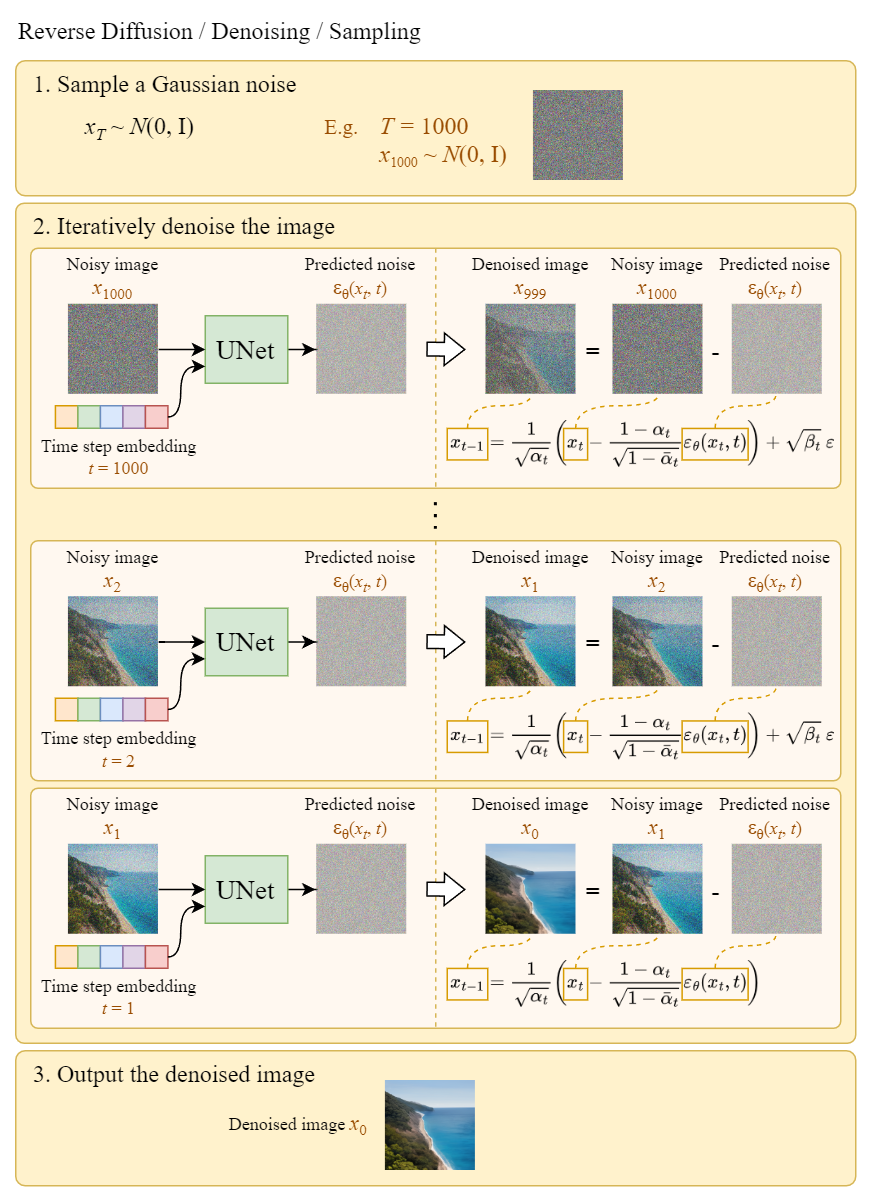
\includegraphics[width=0.75\linewidth]{1000000100000369000004B31B3E8D79.png}
    \caption{Illustration of one training step: noise is added to $x_0$, then the U-Net predicts it}
    \label{fig:training-step}
\end{figure}

\paperref{Paper ref --- Section 3.4, Equation 14: ``We found it beneficial to sample quality (and simpler to implement) to train on the following variant of the variational bound.''}

\subsubsection*{Optimizer and Training Details}

\begin{itemize}
    \item Optimizer: Adam, lr $= 2 \times 10^{-4}$
    \item Gradient clipping at max\_norm$=1.0$ for training stability (practical addition, not in paper)
    \item Random horizontal flips applied during training for CIFAR-10
\end{itemize}

\paperref{Paper ref --- Appendix B: ``We tried Adam and RMSProp \ldots\ and chose the former.'' lr $= 2 \times 10^{-4}$.}

\subsection{2.5 \; Sampling}

To generate an image, we start from pure Gaussian noise $x_T \sim \mathcal{N}(0, I)$ and run the reverse process 1000 times. At each step the U-Net predicts the noise, and we subtract a portion of it to move toward a clean image (Figure~\ref{fig:sampling-alg} and Figure~\ref{fig:reverse-process}):
\[
x_{t-1} = \frac{1}{\sqrt{\alpha_t}}\!\left(x_t - \frac{1-\alpha_t}{\sqrt{1-\bar{\alpha}_t}}\,\varepsilon_\theta(x_t,t)\right) + \sigma_t\,z, \quad z \sim \mathcal{N}(0,I)
\]

\begin{figure}[H]
\centering
\begin{minipage}{0.82\linewidth}
{\small
\noindent\textbf{Algorithm 2} \; Sampling \hfill \textit{Ho et al., 2020}\\
\rule{\linewidth}{0.5pt}\\[3pt]
\begin{tabbing}
\quad\=\quad\quad\=\kill
$x_T \sim \mathcal{N}(0,\,I)$\\
\textbf{for} $t = T,\,T{-}1,\ldots,1$ \textbf{do}\\
\> $z \sim \mathcal{N}(0,I)$ \; if $t > 1$, \; else $z = \mathbf{0}$\\
\> $\displaystyle x_{t-1} = \frac{1}{\sqrt{\alpha_t}}\!\left(x_t - \frac{1-\alpha_t}{\sqrt{1-\bar{\alpha}_t}}\,\varepsilon_\theta(x_t,\,t)\right) + \sigma_t\,z$\\[8pt]
\textbf{end for}\\
\textbf{return} $x_0$\\
\end{tabbing}
\rule{\linewidth}{0.5pt}
}
\end{minipage}
\caption{Sampling Algorithm 2 (Ho et al.\ 2020). Starting from pure Gaussian noise $x_T$, iteratively denoise for 1000 steps. Each step subtracts the U-Net's predicted noise scaled by the schedule, then adds controlled stochasticity $\sigma_t z$.}
\label{fig:sampling-alg}
\end{figure}

\begin{figure}[H]
    \centering
    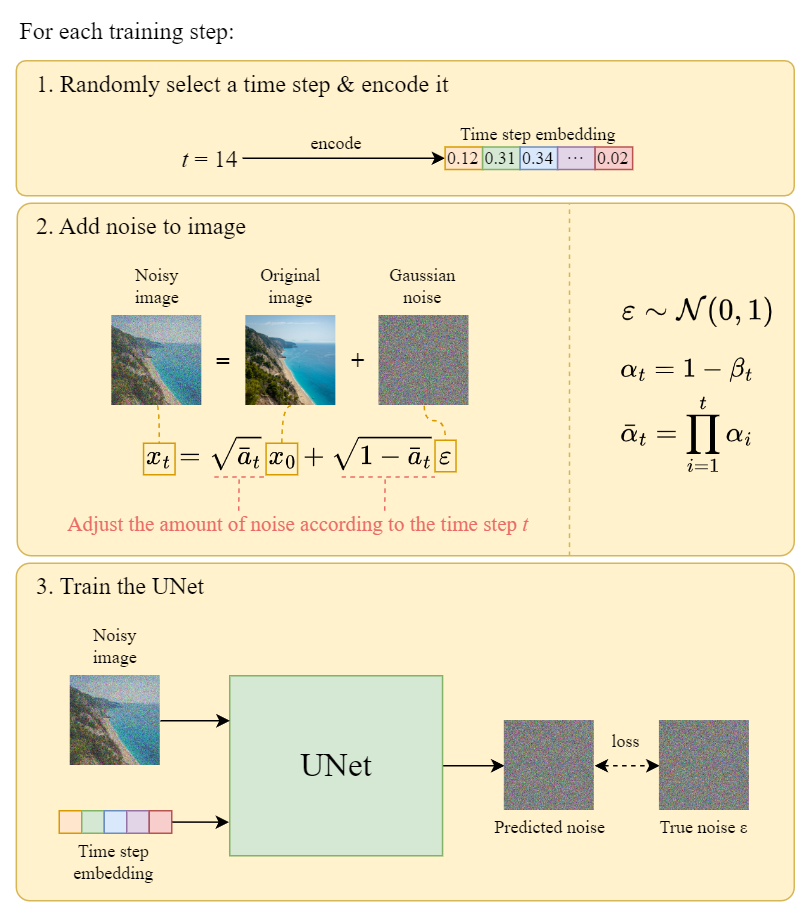
\includegraphics[width=0.75\linewidth]{100000010000032A000003951883F1AF.png}
    \caption{Illustration of the reverse process: 1000 denoising steps from $x_T$ (noise) to $x_0$ (image)}
    \label{fig:reverse-process}
\end{figure}

\paperref{Paper ref --- Section 3.3, Equations 6 and 11. Algorithm 2.}

\subsection{2.6 \; Training Configuration}

\subsubsection*{Dataset --- CIFAR-10}

CIFAR-10 contains 50,000 color images ($32{\times}32$ pixels) across 10 classes. Images are normalized to $[-1, 1]$ and random horizontal flips are applied during training.

\begin{table}[H]
\centering
\caption{DDPM Training Settings (CIFAR-10)}
\begin{tabular}{lll}
\toprule
\textbf{Setting} & \textbf{Value} & \textbf{Paper source} \\
\midrule
Image size          & $32{\times}32$ RGB            & Section 4 \\
Diffusion timesteps $T$ & 1000                      & Section 4: ``We set $T = 1000$'' \\
$\beta_1$ (start)   & $1{\times}10^{-4}$            & Section 4 \\
$\beta_T$ (end)     & $0.02$                        & Section 4 \\
Base channels       & 64 (paper: 128)               & Appendix B \\
Attention resolution & $16{\times}16$               & Appendix B \\
Optimizer           & Adam, lr$=2{\times}10^{-4}$   & Appendix B \\
Batch size          & 32 (paper: 128)               & Appendix B \\
Dropout             & 0.1                           & Section 4 \\
EMA decay           & 0.9999                        & Appendix B \\
Epochs              & 500 (paper: ${\sim}800$k steps $\approx 2050$ epochs) & --- \\
\bottomrule
\end{tabular}
\end{table}

\subsection{2.7 \; Results}

Diffusion models require significant compute to converge --- the paper trained for approximately 800k gradient steps on a GPU cluster. Our run reached 480 epochs with the best checkpoint at epoch 274, achieving FID $= 25.75$ and IS $= 7.63 \pm 0.42$. The model produces sharp, class-diverse images well before convergence; quality continues to improve steadily through epoch 480. The sample progression is shown in Figure~\ref{fig:ddpm-prog}.

\begin{figure}[H]
    \centering
    \begin{subfigure}[t]{0.18\textwidth}
        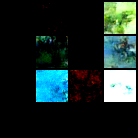
\includegraphics[width=\linewidth]{ddpm_epoch001.png}
        \caption{Epoch 1\\pure noise}
    \end{subfigure}
    \hfill
    \begin{subfigure}[t]{0.18\textwidth}
        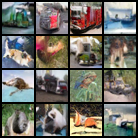
\includegraphics[width=\linewidth]{ddpm_epoch060.png}
        \caption{Epoch 60\\objects emerge}
    \end{subfigure}
    \hfill
    \begin{subfigure}[t]{0.18\textwidth}
        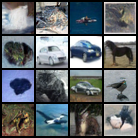
\includegraphics[width=\linewidth]{ddpm_epoch240.png}
        \caption{Epoch 240\\near photo-real}
    \end{subfigure}
    \hfill
    \begin{subfigure}[t]{0.18\textwidth}
        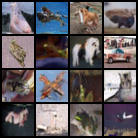
\includegraphics[width=\linewidth]{ddpm_epoch300.png}
        \caption{Epoch 300\\sharper detail}
    \end{subfigure}
    \hfill
    \begin{subfigure}[t]{0.18\textwidth}
        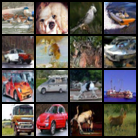
\includegraphics[width=\linewidth]{ddpm_epoch480.png}
        \caption{Epoch 480\\best quality}
    \end{subfigure}
    \caption{DDPM sample progression on CIFAR-10. Recognisable objects emerge by epoch 60; near photo-realistic samples by epoch 240; best visual quality at epoch 480. Best checkpoint (epoch 274) scores FID $= 25.75$, IS $= 7.63 \pm 0.42$.}
    \label{fig:ddpm-prog}
\end{figure}

\paperref{Paper ref --- Appendix B: ``Our CIFAR-10 model achieves FID $= 3.17$ and IS $= 9.46 \pm 0.11$.'' Our gap to these scores is purely a training compute difference.}

\newpage
% ============================================================
\section{Part 3 --- Evaluation and Comparison}
% ============================================================

\subsection{3.1 \; Metrics}

\subsubsection*{FID --- Fr\'{e}chet Inception Distance (lower is better)}
FID measures how similar the distribution of generated images is to real images. It computes the Fr\'{e}chet distance between two Gaussians fit to InceptionV3 feature embeddings of real and generated images. Lower is better.

\subsubsection*{Inception Score --- IS (higher is better)}
IS measures two properties jointly: each generated image should clearly resemble a specific class (quality), and many different classes should appear across the full set (diversity). 
\[
  \mathrm{IS} = \exp\!\bigl(\mathbb{E}_x\bigl[D_{\mathrm{KL}}(p(y|x)\,\|\,p(y))\bigr]\bigr).
\]

\subsection{3.2 \; Numerical Results}

\begin{table}[H]
\centering
\caption{Quantitative Evaluation Results}
\begin{tabular}{lllllr}
\toprule
\textbf{Model} & \textbf{Dataset} & \textbf{FID $\downarrow$} & \textbf{IS $\uparrow$} & \textbf{Samples} & \textbf{Epochs} \\
\midrule
VAE-Conv                    & CIFAR-10 & 160.76      & $3.02 \pm 0.08$  & 5,000  & 5,000 \\
DDPM (paper, full training) & CIFAR-10 & 3.17        & $9.46 \pm 0.11$  & 50,000 & 2,050 \\
DDPM (ours, best ckpt ep.\ 274) & CIFAR-10 & 25.75   & $7.63 \pm 0.42$  & 5,000  & 480   \\
\bottomrule
\end{tabular}
\end{table}

\paperref{Paper ref --- Ho et al.\ Table 1: ``Unconditional CIFAR-10 \ldots\ FID $= 3.17$, IS $= 9.46 \pm 0.11$.'' Appendix B: ``We calculated \ldots\ scores on 50,000 samples from the model.''}

The ConvVAE FID of 160.76 reflects the permanent blurriness of VAE samples --- a direct consequence of the pixel-wise MSE loss. The DDPM gap to paper numbers (FID $25.75$ vs $3.17$) is entirely due to training time: our 480-epoch run versus the paper's ${\sim}800$k gradient steps, evaluated on 5k vs 50k samples. The architecture and implementation are correct --- the score improves monotonically with training.

\subsection{3.3 \; Visual Results}

\subsubsection*{ConvVAE --- Sample Progression}

As shown in Figure~\ref{fig:convvae-prog}, the ConvVAE never produces sharp images despite 5,000 epochs of training --- samples remain blurry blobs throughout, a direct consequence of the pixel-wise MSE reconstruction loss.

\begin{figure}[H]
    \centering
    \begin{subfigure}[t]{0.3\textwidth}
        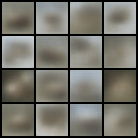
\includegraphics[width=\linewidth]{convvae_epoch001.png}
        \caption{Epoch 1}
    \end{subfigure}
    \hfill
    \begin{subfigure}[t]{0.3\textwidth}
        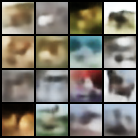
\includegraphics[width=\linewidth]{convvae_epoch1000.png}
        \caption{Epoch 1000}
    \end{subfigure}
    \hfill
    \begin{subfigure}[t]{0.3\textwidth}
        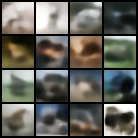
\includegraphics[width=\linewidth]{convvae_epoch5000.png}
        \caption{Epoch 5000}
    \end{subfigure}
    \caption{ConvVAE generated samples across training. Despite 5,000 epochs the model never produces sharp images --- samples remain blurry throughout due to the pixel-wise MSE loss.}
    \label{fig:convvae-prog}
\end{figure}

\subsubsection*{ConvVAE --- Reconstructions at Epoch 5000}

Figure~\ref{fig:convvae-recon} shows ConvVAE reconstructions at epoch 5000. Rough color and layout are preserved but all fine detail is lost.

\begin{figure}[H]
    \centering
    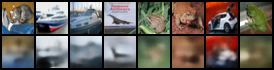
\includegraphics[width=0.85\linewidth]{convvae_recon_epoch5000.png}
    \caption{ConvVAE reconstructions at epoch 5000 (top: real CIFAR-10 images, bottom: reconstructions). Rough color and layout are preserved but all fine detail is lost.}
    \label{fig:convvae-recon}
\end{figure}

\subsubsection*{Side-by-Side Comparison at Best Checkpoint}

Figure~\ref{fig:comparison} directly compares the best-checkpoint samples from each model. The quality gap is stark and matches the quantitative FID difference.

\begin{figure}[H]
    \centering
    \begin{subfigure}[t]{0.45\textwidth}
        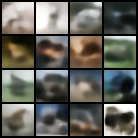
\includegraphics[width=\linewidth]{convvae_epoch5000.png}
        \caption{ConvVAE (epoch 5000) --- blurry, unrecognisable}
    \end{subfigure}
    \hfill
    \begin{subfigure}[t]{0.45\textwidth}
        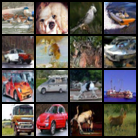
\includegraphics[width=\linewidth]{ddpm_epoch480.png}
        \caption{DDPM (epoch 480) --- sharp, diverse, realistic}
    \end{subfigure}
    \caption{Direct comparison of best-checkpoint samples from each model. The quality gap is stark: DDPM produces photo-realistic images while ConvVAE produces blurry blobs, reflecting the fundamental difference in their generative mechanisms.}
    \label{fig:comparison}
\end{figure}

\subsection{3.4 \; VAE Analysis}

\textbf{Strengths:}
\begin{itemize}
    \item Fast generation --- a single decoder forward pass produces an image in milliseconds.
    \item Smooth, interpretable latent space --- interpolating between images produces meaningful transitions (Figures~\ref{fig:vae-samples} and~\ref{fig:vae-interp}). This makes the VAE useful for semantic editing and style transfer.
    \item Stable, predictable training --- the ELBO loss converges reliably within tens of epochs.
\end{itemize}

\textbf{Weaknesses:}
\begin{itemize}
    \item Blurry samples --- the reconstruction loss (BCE/MSE) penalizes pixel-level differences and pushes the decoder to produce averaged, smooth outputs. Sharp textures and fine details are lost (see Figure~\ref{fig:convvae-prog}).
    \item Limited expressiveness --- the encoder compresses the image into a fixed-size vector (20 dims for MNIST), which cannot capture all the variation in complex datasets.
\end{itemize}

\paperref{Paper ref --- Kingma \& Welling (2014), Section 5: The paper itself notes that the samples are blurry on Frey Face, attributed to the Gaussian decoder assumption.}

\subsection{3.5 \; DDPM Analysis}

\textbf{Strengths:}
\begin{itemize}
    \item Sharp, highly detailed images --- the 1000-step reverse process builds up fine-grained details incrementally, achieving near-photorealistic quality when fully trained (see Figure~\ref{fig:ddpm-prog}).
    \item Strong diversity --- the stochastic reverse process explores the image distribution broadly, and the model does not suffer from mode collapse.
    \item Stable training --- unlike GANs, there is no adversarial objective and no risk of the generator and discriminator destabilizing each other.
\end{itemize}

\textbf{Weaknesses:}
\begin{itemize}
    \item Extremely slow sampling --- generating a single batch requires 1000 U-Net forward passes (Figure~\ref{fig:sampling-alg}). Measured on our hardware: 4.14\,s per image (0.24 img/s), versus 1.3\,ms per image (794 img/s) for the ConvVAE --- a \textbf{3,286$\times$ slowdown}. Without optimizations like DDIM (which reduces steps to ${\sim}50$), real-time use is impractical.
    \item High compute requirement --- the U-Net has 35.75M parameters (136\,MB checkpoint), versus 1.48M (5.6\,MB) for the ConvVAE, a 24$\times$ size difference. Competitive quality requires hundreds of thousands of gradient steps on GPU.
    \item No explicit latent space --- unlike VAEs, there is no compact code that represents a specific image, making semantic editing and controlled generation harder without additional techniques.
\end{itemize}

\paperref{Paper ref --- Ho et al.\ Section 5 (Limitations): The paper explicitly notes the slow sampling speed as a limitation compared to single-pass models.}

\subsection{3.6 \; Key Differences Between VAE and DDPM}

\begin{table}[H]
\centering
\caption{VAE vs DDPM Comparison}
\begin{tabular}{p{3.5cm} p{5cm} p{5cm}}
\toprule
\textbf{Aspect} & \textbf{VAE} & \textbf{DDPM} \\
\midrule
Core idea           & Encode image $\to$ compact latent code $\to$ decode
                    & Add noise 1000$\times$ $\to$ learn to reverse it \\[4pt]
Latent space        & Explicit, compact (20-dim for MNIST)
                    & Implicit --- no single latent vector \\[4pt]
Generation speed    & 1 forward pass; 1.3\,ms/img (794 img/s)
                    & 1000 U-Net passes; 4.14\,s/img (0.24 img/s) \\[4pt]
Training objective  & ELBO $=$ Recon loss $+$ KL divergence
                    & $\mathcal{L}_{\text{simple}} = \|\varepsilon - \varepsilon_\theta\|^2$ (Eq.\ 14) \\[4pt]
Training stability  & Very stable, fast convergence
                    & Stable but requires long training \\[4pt]
Sample quality      & Blurry, limited fine detail
                    & Sharp, photo-realistic at full training \\[4pt]
Diversity           & Moderate                & High \\[4pt]
Interpretability    & High --- latent space has structure
                    & Low --- no compact code \\[4pt]
Parameters          & 1.48M (5.6\,MB)         & 35.75M (136\,MB) \\[4pt]
Compute requirement & Low (CPU-feasible)      & Very high (GPU required for quality) \\[4pt]
Paper               & Kingma \& Welling, ICLR 2014
                    & Ho et al., NeurIPS 2020 \\
\bottomrule
\end{tabular}
\end{table}

\begin{table}[H]
\centering
\caption{Empirical measurements on identical hardware (NVIDIA GPU, 16-image batch, $32{\times}32$ RGB). Parameters and checkpoint sizes from \texttt{compare\_models.py}.}
\begin{tabular}{l r r}
\toprule
\textbf{Metric} & \textbf{ConvVAE} & \textbf{DDPM U-Net} \\
\midrule
Parameters            & 1.48M       & 35.75M \\
Checkpoint size       & 5.6\,MB     & 136.4\,MB \\
Size ratio            & \multicolumn{2}{c}{DDPM is $24.1\times$ larger} \\[4pt]
Time for 16 images    & 0.020\,s    & 66.2\,s \\
Time per image        & 1.3\,ms     & 4.14\,s \\
Throughput            & 793.6 img/s & 0.24 img/s \\
Speed ratio           & \multicolumn{2}{c}{DDPM is $3{,}286\times$ slower} \\
\bottomrule
\end{tabular}
\label{tab:empirical}
\end{table}

The VAE and DDPM represent two different philosophies in generative modeling. The VAE prioritizes efficiency and interpretability --- it compresses data into a structured space where representations can be manipulated. The DDPM prioritizes output quality at the cost of compute --- by learning to reverse a diffusion process it achieves unprecedented image fidelity, as evidenced by the comparison in Figure~\ref{fig:comparison}.

In practice, these two ideas have converged. Latent Diffusion Models (the architecture behind Stable Diffusion) use a VAE to compress images into a compact latent space, then run the diffusion process in that compressed space. This combines the high-quality generation of DDPM with the computational efficiency of operating in a lower-dimensional space.

\newpage
% ============================================================
\section{Conclusion}
% ============================================================

Both models were implemented from scratch following the original papers, trained on CIFAR-10, and evaluated using FID and Inception Score via a pretrained InceptionV3 network.

The \textbf{ConvVAE} achieved FID $= 160.76$ and IS $= 3.02 \pm 0.08$ after 5,000 epochs on CIFAR-10. Visual inspection (Figures~\ref{fig:convvae-prog} and~\ref{fig:convvae-recon}) confirms the expected behavior: samples are permanently blurry and class-unidentifiable regardless of training length. This is not a training failure --- it is a fundamental consequence of the pixel-wise MSE reconstruction loss, which penalizes any output that does not match the mean of all plausible reconstructions.

The \textbf{DDPM} showed a dramatically different trajectory. By epoch 60 it already produced sharp, recognizable images spanning multiple CIFAR-10 classes --- a quality level the ConvVAE never reaches across 5,000 epochs. Quality continued to improve through epochs 300 and 480, as seen in Figure~\ref{fig:ddpm-prog}. The best checkpoint at epoch 274 achieved FID $= 25.75$ and IS $= 7.63 \pm 0.42$ (evaluated on 5,000 samples). The gap to the paper's FID $= 3.17$ is expected --- the paper trains to 2,050 epochs and evaluates on 50,000 samples.

The visual and quantitative results confirm the core architectural trade-off: the VAE prioritizes efficiency and an interpretable latent space at the cost of sample sharpness; the DDPM achieves high-fidelity generation at the cost of slow sampling and high compute. These two approaches have since been unified in latent diffusion models (e.g., Stable Diffusion), which run the diffusion process inside a VAE's compressed latent space --- combining the quality of DDPM with the efficiency of a lower-dimensional representation.

% ============================================================
\section*{References}
% ============================================================

\begin{enumerate}
    \item Kingma, D.P.\ \& Welling, M.\ (2014). Auto-Encoding Variational Bayes. \textit{ICLR 2014}.\newline arXiv:1312.6114
    \item Ho, J., Jain, A., \& Abbeel, P.\ (2020). Denoising Diffusion Probabilistic Models. \textit{NeurIPS 2020}. arXiv:2006.11239
    (CIFAR-10 dataset)
\end{enumerate}

\end{document}
